\chapter{Data samples and simulation}
\begin{section}{Data}

The dataset used in this search corresponds to 35.9~\ifb of proton-proton collisions at $\sqrt{s} = 13~\TeV$ collected by the CMS detector over the year 2016.
This is a subset of the 40.8~\ifb delivered by the LHC and selected to correspond to when all sub-detectors were fully-operational.
A plot of the cumulative delivered and recorded integrated luminosity by the LHC and CMS, respectively, is shown in~\ref{fig:lumi_2016}. 

\begin{figure}[tbp!]
\begin{center}
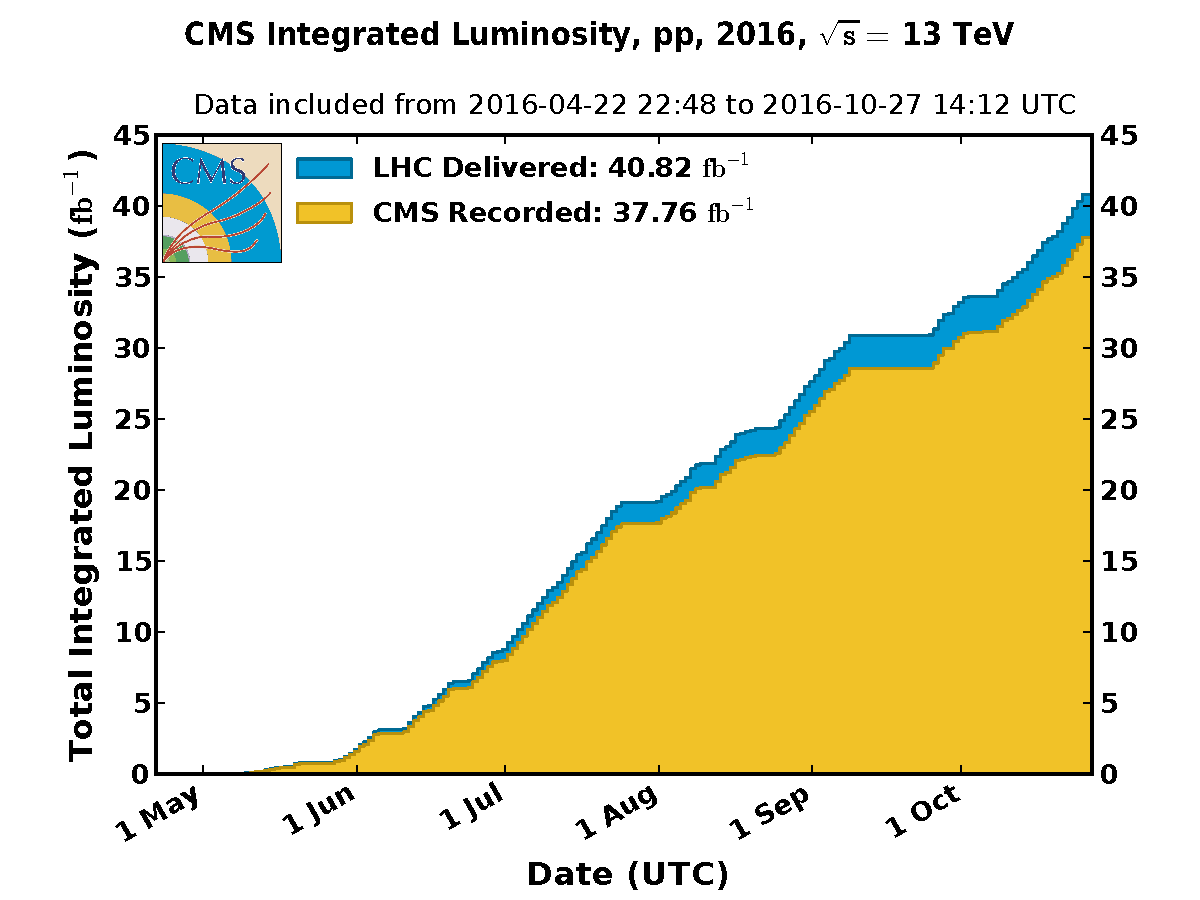
\includegraphics[angle=0,width=0.95\columnwidth]{fig/lumi_2016.pdf}
\end{center}
\caption{Delivered and recorded integrated luminosity by the LHC and CMS, respectively, over 2016.~\cite{lumi_2016}}
\label{fig:lumi_2016}
\end{figure}

\end{section}

\begin{section}{Monte Carlo Simulation}

Simulated samples are used to model both SM and BSM physics processes, and are extremely useful in the design and execution of new physics searches.
In this particular analysis the Monte Carlo simulations (MC) are used to in the following ways:
\begin{itemize}
\item Design and optimization of the analysis strategy
\item Validation of (signal-plus-)background prediction methods
\item Study of processes with impure and/or statisticallly small control regions
\item Commissioning and understanding of collected data
\item Modelling BSM physics processes that may or may not exist
\end{itemize}

\MGatNLO 2.2.2 is used in leading-order mode~\cite{Alwall:2014hca,Alwall:2007fs} to generate the
\ttbar, \Wjets, quantum chromodynamics multijet (QCD), and Drell--Yan background processes with extra partons.
Comparison to a \POWHEG 2.0~\cite{Nason:2004rx,Frixione:2007vw,Alioli:2010xd} sample generated at next-to-leading order (NLO) shows
that the NLO effects do not have a significant impact.
The \ttW, \ttZ, \tttt, and $t$-channel single top quark production backgrounds
are generated with \MGatNLO 2.2.2 in NLO mode~\cite{Frederix:2012ps}, while
the $\mathrm{tW}$, $\mathrm{\bar{t}W}$, and $s$-channel single top quark processes are generated with \POWHEG~2.0.
The \ttbar, \Wjets, and QCD samples are generated with up to 2, 4, 2 extra partons, respectively.
All samples are generated using a top quark mass of 172.5 \GeV and with the NNPDF3.0 set of parton distribution functions (PDF)~\cite{Ball:2014uwa}.
For the fragmentation and showering of partons, the generated samples are interfaced with \PYTHIA~8.205~\cite{pythia8.2} and use the CUETP8M1 tune to describe the underlying event~\cite{Skands2014}.
All samples use the highest precision cross sections available~\cite{PhysRevLett.110.252004,Gavin:2012sy,Alioli:2009je,Re:2010bp,Frixione:2015zaa,Bevilacqua:2012em,Nagy:2001fj}.
The detector response is simulated with \GEANTfour~\cite{Agostinelli:2002hh}.
Simulated samples are processed through the same reconstruction algorithms as the data.

The signal samples are generated with up to two extra partons in leading-order mode and dynamic factorization and renormalization scales by \MGatNLO~2.2.2.
The same fragmentation, parton showering, simulation, and event reconstruction procedure as for the background samples is used.
The samples are normalized to NLO + next-to-leading logarithmic cross sections~\cite{XSecgluinogluino}.

\end{section}

%%%% NOTES
% 1. Talk about simplified models and the details about the signal model.
